\documentclass[pdf]{beamer}
\usepackage[latin1]{inputenc}
\usepackage{multirow}
\usetheme{Antibes} %Warsaw
\usecolortheme{wolverine}


\begin{document}

\title[Experimental Design]{Experimental Design}
\subtitle{BCB 504: Applied Bioinformatics\\}
\author[Matt Settles]{Matt Settles}
\institute{University of Idaho\\ Bioinformatics and Computational Biology Program}
\date{\today}


%% Title page
\begin{frame}[plain]
  \titlepage
\end{frame}


%% Outline
\begin{frame}[plain] 
  \frametitle{Outline}
  \tableofcontents
\end{frame}

\section{Sample Preparation}
\begin{frame}
\frametitle{Sample Preparation}
In high throughput biological work (Microarrays, Sequencing, HT Genotyping, etc.), what may seem like small technical artifacts introduced during sample extraction/preparation can lead to large changes, or bias, in the data. Not to say this doesn't occur with smaller scale analysis such as Sanger sequencing or rtPCR, but they do become more appart and may cause significant issues during analysis.
\end{frame}


\begin{frame}
\frametitle{Sample Preparation}
Some suggestions
\begin{enumerate}
\item Prepare more samples then you are going to need, ie expect some will be of poor quality.
\item Preparation stages should occur across all samples at the same time (or as close to) and by the same person.
\item Spend time practicing to produce the highest quality product you can.
\item Quality and quantity should be established using Bioanalyzer traces (pseudo-gel images), 260/280 \& 260/230 $>$ 1.8, and quantified by fluourametry.  
\item RNA should not be degrated, Bioanalyzer give RIN numbers to measure relative degradation. 
\end{enumerate}
\end{frame}

\begin{frame}
\frametitle{Sample Preparation}
The GRC likes to see a minimum RIN value of XX.
\begin{center}
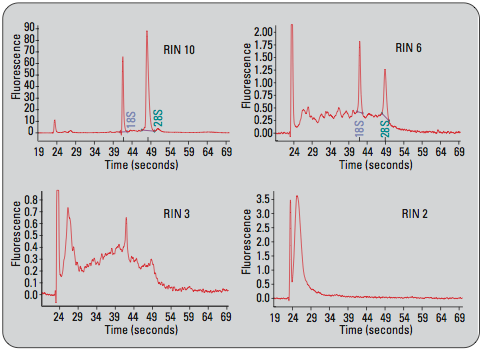
\includegraphics[scale=0.50]{Figures/RIN.png} 
\end{center}
\end{frame}

\section{Coverage}
\begin{frame}
\frametitle{How much coverage do you need (assembly)}
    Idealized Lander-Waterman model (1988)
    \begin{footnotesize}
    \begin{itemize}
    \item Reads start at perfectly random position
    \item Poisson distribution in coverage
    \item Contig length is a function of coverage and read length
    \end{itemize}
	\end{footnotesize}
the probability a base is not sequenced is given by: $P_0 = e^{-c}$\\
where $e = 2.718$, $c$ = fold sequence coverage\\
$c = LN/G$\\
$L = $ read length, $N = $ number of reads, $G = $ genome size.\\
Formula used for the original Human Genome project.\\

\alert{Does not consider read error rate, or genome complexity. Only probability of sequencing a base.} \\

Roach \href{http://genome.cshlp.org/content/5/5/464.long}{1995} published an expanded theory.\\

\end{frame}

\begin{frame}
\frametitle{Lander-Waterman model}
\begin{center}
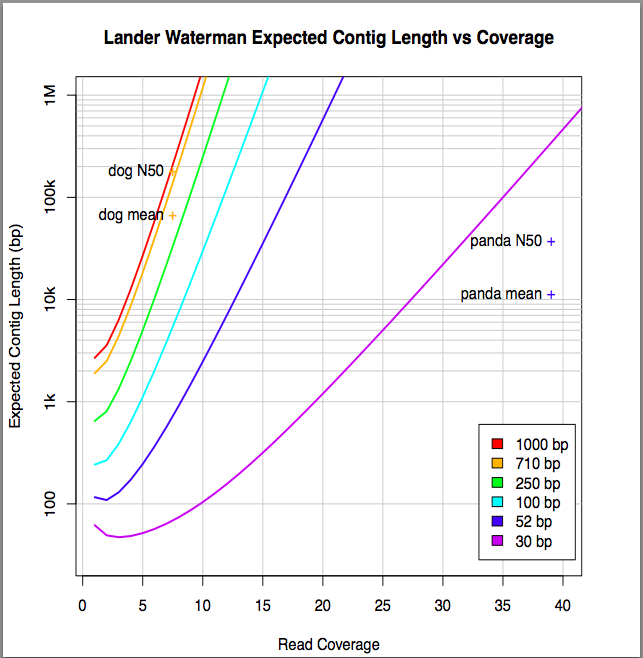
\includegraphics[scale=0.30]{Figures/coverage.png} 
\end{center}
\end{frame}

\begin{frame}
\frametitle{Practical Size Considerations}
\begin{center}
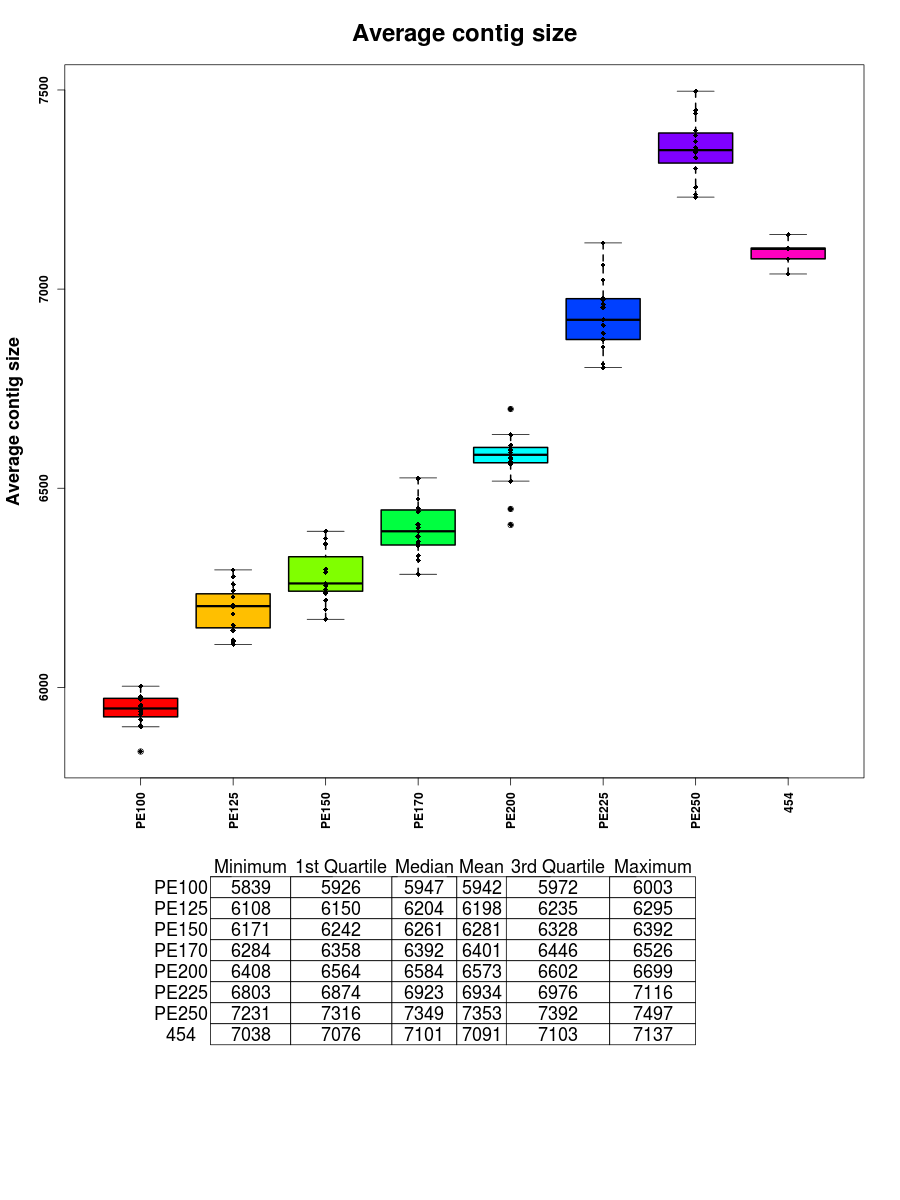
\includegraphics[scale=0.19]{Figures/avgContigSize.png} 
\end{center}
\end{frame}

\begin{frame}
\frametitle{Example Genome Assembly Approach}
Approach published Jan. 2012, crocodilian genome, expected completion Jun. 2012. (estimated genome size ~2.75Gb.) 
\begin{itemize}
\item 50x coverage from an overlapping, Illumina, short-insert library.
\item 20x coverage from an Illumina 2kb mate-pair library.
\item 50x coverage from a non-overlapping 2x100bp, Illumina, short-insert library.
\item 1x coverage from a 700bp, 454 library
\item 2x coverage from a 3kb and 6kb, 454 library
\item BAC end sequencing
\item Finally, FISH mapping the BACs to assign scaffolds to chromosomes.
\end{itemize}
\alert{No updates on progress since then, though data is being updated}
\end{frame}

\begin{frame}
\frametitle{Coverage by sequencing run}
Determine run data (\href{http://www.illumina.com/systems/hiseq_2500_1500/performance_specifications.ilmn}{Illumina specs}).
\vspace{0.2in}
Get read (or bp) per lane = \\
Dual Flow Cell / 16
\\
Single Flow Sell / 8\\

Est. Coverage then is: $(readsLane*readLength)/(genomeSize*numberOfSamples)$\\
\vspace{0.2in}
I usually use low estimate for reads (or bp) and then multiple Est. Coverage by 0.8 for quality. \\
\vspace{0.2in}
Also know actual equal proportions between multiplexed samples is rare and can be multiple fold off.\\
\end{frame}

\begin{frame}
\frametitle{Bottom Line}
Bottom Line:\\
Spend the time (and money) producing good quality, accurate and sufficient data for your experiment. You will spend much more time (and more dollars) trying to pull out biological significant and results in bioinformatic analysis. 
\end{frame}

\end{document}
